\section{Logistics}
\label{sec:fdsp-tc-log}
% \cite{bib:docdb8255}

Access to the underground installation area for \dword{dune},   \dword{lbnf}, and \dword{jpo} personnel, as well as for  \dword{lbnf} and \dword{dune}  materials and equipment, will be provided by a single shaft, the \SI{1500}{m}-deep Ross Shaft. Coordinating transport and ensuring on-time delivery of all items are therefore among the more challenging aspects of the \dword{lbnf} and \dword{dune} endeavor. 
The \dword{jpo} (see Volume~\volnumbertc~\voltitletc, Chapter~\ref{ch:tc-jpo} of this \dword{tdr}) will establish a logistics organization for \dword{lbnf} and \dword{dune}, operated under the Fermilab \dword{sdsd}, to verify deliveries to the point of receipt in South Dakota and coordinate transport of materials from there  to the Ross Headframe.  \fixme{check TC vol ref; and last sentence - correct? Anne} 


Due to the enormous cost of the \dword{lbnf}-\dword{cf} contracts and the risk of increased construction costs due to delays in delivery of materials, the shaft scheduling must be tightly controlled by \dword{lbnf}-\dword{cf} during construction.
The shaft is outfitted with a hoists that control the cage and skips. The cage is used to transport people, equipment and materials, and the skips to bring up muck and transport over-sized equipment and materials. The \dword{lbnf}-\dword{cf} \dword{cmgc} will coordinate overall usage of the Ross Shaft during this period.


To facilitate the flow of (non-\dword{cf}) \dword{lbnf} and \dword{dune} materials and equipment to the Ross Headframe, the \dword{jpo} will lease a warehouse facility within a maximum one-day roundtrip from \dword{surf} by truck. 
It is expected that the lease of this facility, referred to as the \dword{sdwf}, will include warehouse space, personnel and a \dword{wms} to inventory all incoming materials and equipment. 
A facility has not yet been selected. 


Most materials and equipment will be shipped to the \dword{sdwf}; \dword{cf} material, and likely cryogenics equipment, are exceptions and will ship directly to \dword{surf}. 
The \dword{sdsd} logistics  organization will (1) receive and inventory all  goods shipped to the \dword{sdwf}, (2) coordinate with the \dword{cf}-\dword{cmgc}  and transport this material to the Ross Headframe in a just-in-time manner, and (3) transport it underground and into the cavern. 
Figure~\ref{fig:logistics-material-flow} shows a high-level overview of the material flow to the Ross Headframe.

 
\begin{dunefigure}[Material flow diagram for \dword{lbnf} and \dword{dune}]
{fig:logistics-material-flow}
  {Material flow diagram for \dword{lbnf} and \dword{dune}. }
 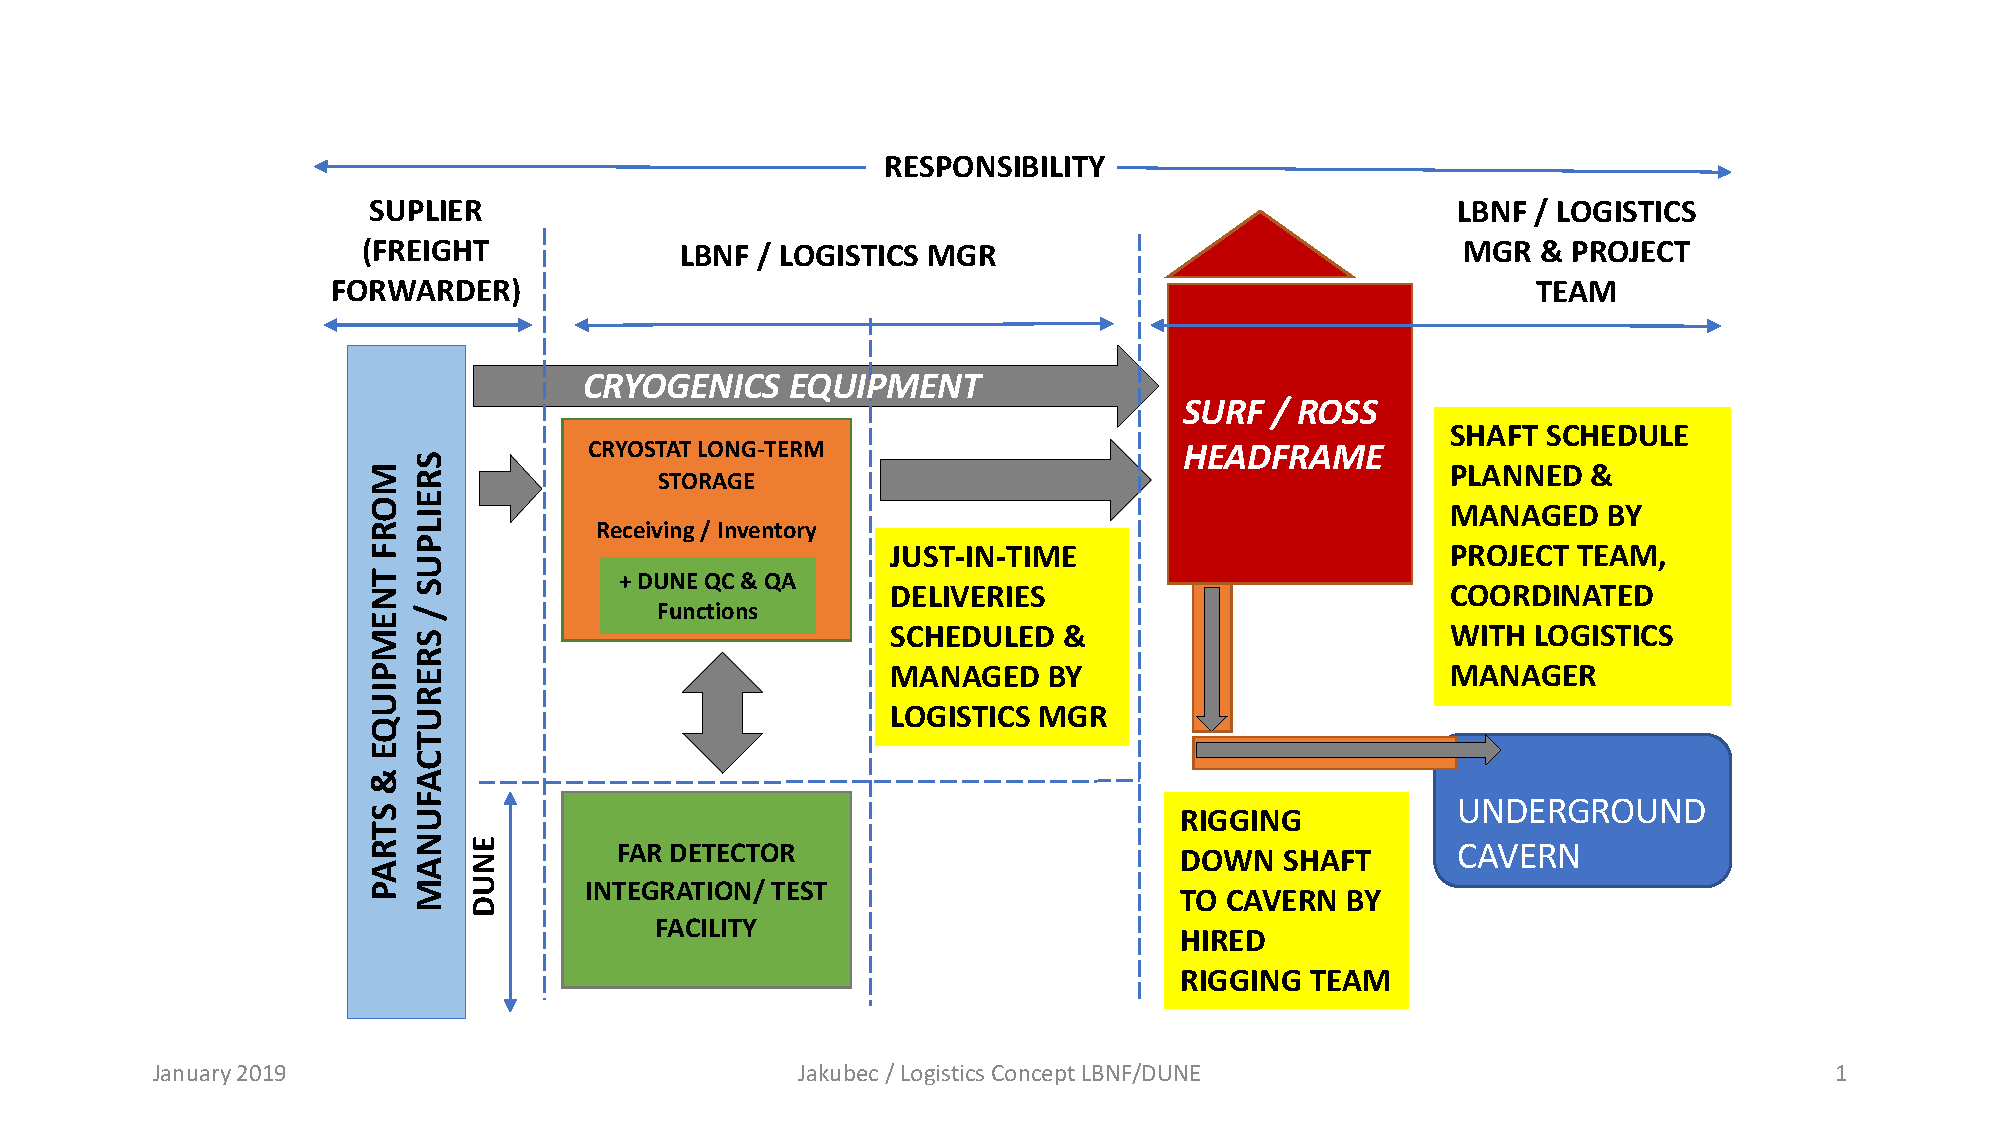
\includegraphics[width=\textwidth]{logistics-material-flow}
\end{dunefigure}

%%%%%%%%%%%%%%%%%%%%%%%%%%%%  
\subsection{Logistics Planning}
\label{sec:fdsp-tc-logPln}

The \dword{jpo}/\dword{sdsd} logistics team oversees transportation of the cryostat (steel, foam, and membrane), the cryogenics system, the \dword{dune} detector components, and all related infrastructure not provided by the \dword{cf}. 
\fixme{As I understand it the logistics personnel are employed by the sdsd but directed by the JPO. If Patrick agrees this is the case then the first sentence needs to reflect this. Jim}
\dword{lbnf} specifically oversees the cryostat and cryogenics system, which are  discussed in detail in the \dword{lbnf} \dword{tdr}; because \dword{lbnf} material dominates the logistics, we present a summary.  
 \fixme{Anne needs to add LBNF TDR ref when available}
The steel structure for a \dword{dune} cryostat requires roughly 1,800 individual steel pieces,  some of which weigh up to \SI{7.5}{t}, as well as \SI{125}{t} of bolts to assemble the steel frame. 
The internal structure for the cryostat, which includes the foam insulation and the thin stainless steel membrane, requires transporting roughly 4,000 boxes of approximate size  1.5 $\times$ 3.5 $\times$ 1.2 m$^3$. 
 The current plan calls for warehousing all these boxes at the \dword{sdwf} before installation begins. 
The logistics operation will require roughly $\SI{5000}{m^2}$ of space available approximately two years before installation of the first \dword{detmodule} begins. 
By the time detector components start arriving, most of the cryostat boxes will have been delivered to \dword{surf}, leaving ample space for the detector and the cryogenics components. 
Additional space may be required if the boxes for the second cryostat arrive before  \dword{detmodule} \#1 installation is complete; a few buildings of the required size are available in the general area around \dword{surf}. 

\begin{dunefigure}
[Simplified model of the Ross Cage]
{fig:fdsp-tc-Cage}
{Simplified Ross Cage model and Specifications.}
\parbox{2.1in}{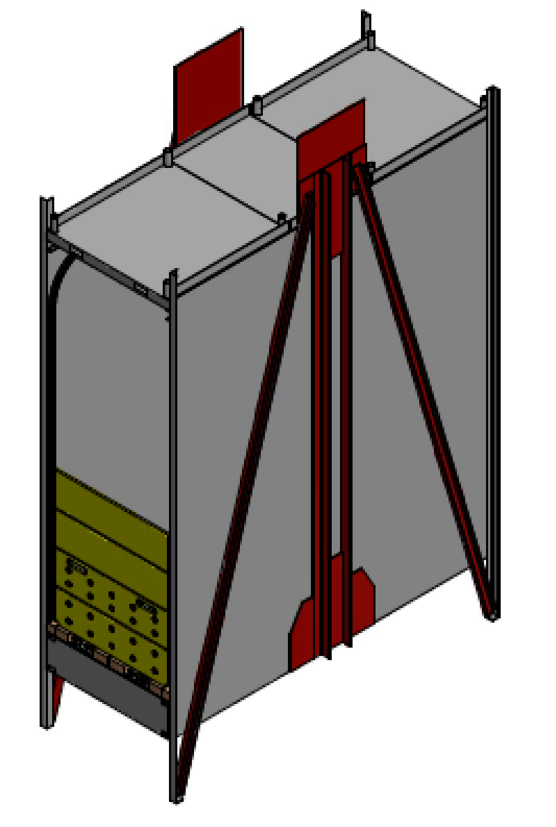
\includegraphics[width=0.3\textwidth]{graphics/Cage-view.pdf}}
\qquad\hspace{10pt}
\begin{minipage}{0.5\textwidth}%
\begin{tabular}{p{3.4cm}p{3.4cm}}        
\multicolumn{2}{c}{Ross Cage Specifications}\\ \toprowrule
Inside height & 3.6 m\\ \colhline
Inside depth  & 3.7 m \\ \colhline
Inside width  & 1.38 m \\ \colhline
Weight limit  &  5,897 kg \\ \colhline
Round trip \newline time & 17 min \newline (incl. unloading) \\ \colhline
\end{tabular}
\end{minipage}
\end{dunefigure}

The \dword{surf} Facility Access Specification~\cite{bib:docdb328} defines the limitations on dimensions and weights for all materials to be transported underground, the most stringent of which are set by the Ross Shaft and Cage. 
It is possible to bring material down the shaft underneath the cage or in the skip compartment  as a slung load, but this is a much slower process and requires careful planning %detailed procedures, and review. 
and review of detailed procedures for each trip. 
The  \dword{apa}s, for example, require this special handling because they are too tall to fit in the cage. 

Most material will be brought underground inside the cage. Figure~\ref{fig:fdsp-tc-Cage} illustrates the new Ross Cage and summarizes its parameters.  
The roundtrip travel time for the Ross cage is 17 minutes (actual travel time is \num{3.6} minutes each way), dominated by loading and unloading time.  
Slung loads will require more than an hour round trip.



The Ross Headframe has no loading dock so careful planning of material loading and unloading of shipments is required. 
All materials must arrive at \dword{surf} on a flatbed or curtain-sided chassis, and a forklift will be available for unloading. 
All deliveries, either from the \dword{sdwf} or direct to the Ross Headframe, require (1) coordination with the logistics organization, and (2) minimum two weeks prior notice, per an advance delivery plan.  
 
Logistics will provide a shipping manual \cite{bib:docdb13954} to \dword{dune} institutions that  
will specify guidelines on required shipping data and cargo consignment such that the logistics organization can monitor shipping progress and no delays occur due to incomplete or missing documentation. 


In \dword{pdsp}, delays in shipping and customs resulted in up to three weeks delay in the arrival of some parts, which necessitated significant re-planning of the installation work.  To prevent this from becoming a much larger problem in \dword{dune}, we plan a minimum one month buffer of materials. This buffer will allow advance planning for the underground work, with confidence that all materials will be available as needed. 

Sufficient space must be made available at the \dword{sdwf} and in the underground area  to house this material.
The \dword{sdwf} staff will de-consolidate or consolidate arriving cargo into appropriately sized boxes and crates, as needed, for delivery to \dword{surf}, to make the most efficient use of available trucks and the Ross Shaft. 

\begin{dunefigure}[Planned usage of underground space during installation setup]{fig:fdsp-tc-setup}
  {CAD image showing the empty half of the north cavern as used during the installation setup phase of the first \dword{detmodule}.  Half of this empty space will be used for the cryostat work and half for storage of the detector infrastructure. The material shown outside the cavern must be stored in the \dword{sdwf}.}
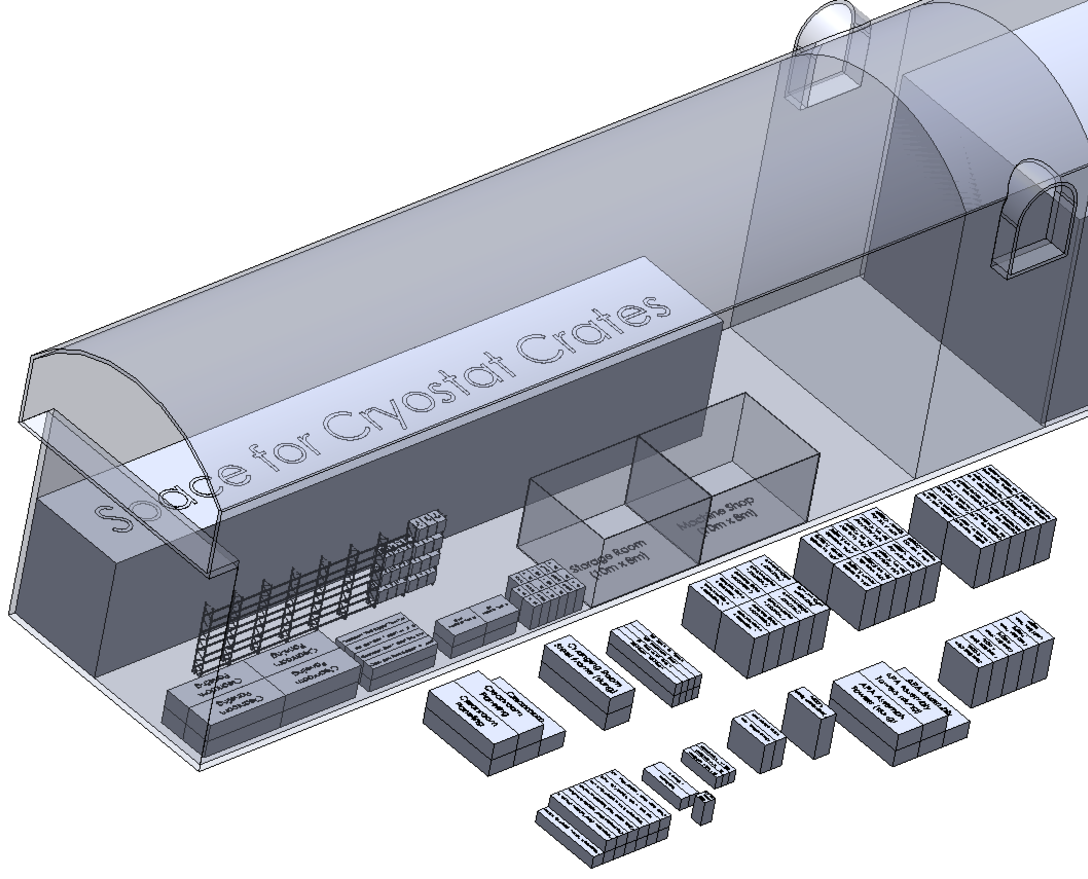
\includegraphics[width=.9\textwidth]{Material-Setup}
\end{dunefigure}


To determine the storage space requirements and how much hoist time must be dedicated to \dword{dune}, a detailed inventory of all  \dword{dune} detector equipment and infrastructure is needed. 
A complete list of materials has been solicited from all consortia and technical coordination. 
The entries in the inventory spreadsheet are organized as \textquotedblleft loads\textquotedblright \ for the Ross shaft where a load is a crate or set of boxes that will be transported underground in one trip, either in the cage or as a slung load~\cite{bib:docdb8426}. 
Information captured in the load spreadsheet includes the number of  
trips, type of trip (slung load or cage), package dimensions, weight, and type of package (crate, pallet, box, or carton). 

The load list at present predicts 1,600 hoist trips and approximately two  months of cage time, most of which is spread over one year. 
Detector installation (see Figure \ref{fig:high-level-schedule}) for the \dword{spmod} will span two years, so we divide the logistics planning into three phases (summarized in Section~\ref{sec:sp-iic-sched}): (1) the \dword{cuc} setup phase, (2) the installation setup phase, and (3) the detector installation phase. 
For each phase, a \threed model was generated to show how much material can be stored underground outside the work area and how much material must be stored 
at the \dword{sdwf}, thus setting the surface space requirements. 
The phase with the largest amount of material to transport is the installation setup phase.  
Figure~\ref{fig:fdsp-tc-setup} shows the model of the underground area and the required boxes for surface storage for the first month of this phase. 
Roughly $\SI{1000}{m^2}$ of warehouse space will be needed at this time.  The \dword{sdwf} will also need space to store up to 150 \dword{apa}s, adding another $\SI{700}{m^2}$. 


%%%%%%%%%%%%%%%%%%%%%%%%%%%%
\subsection{Logistics Quality Control}
\label{sec:fdsp-tc-log-qaqc}


 
The \dword{pdsp} experience offers a couple of significant lessons regarding logistics.

\begin{enumerate}
\item A central inventory system is essential for tracking  shipments.
\item It is important to avoid delays in shipping because they prevent installation work from  proceeding as planned. 
\end{enumerate}

The central inventory system  implemented at the \dword{sdwf}  and minimum one-month material buffer are the plans we have in place to prevent repetition of the \dword{pdsp} schedule problems. 
The full list of lessons learned from \dword{pdsp} is in~\cite{bib:docdb8255}. 

We do not foresee any component testing at the \dword{sdwf}, so the scope of the \dword{qc} work there is limited to two functions: 
The logistics organization in coordination with the the \dword{sdwf} will inventory all received shipments and  ensure that all materials fit in the Ross Cage, or if a slung load is needed, that the necessary procedures are in place and approved before any material is transported to the Ross Headframe.  
\dword{jpo} representatives will verify that no obvious damage occurred in transport. 

The contribution-in-kind model of this project complicates logistics oversight and inventory control 
since components will be delivered from many institutions and from different countries. 
Similarly, during production and testing, \dword{qc} information must be gathered from and made accessible to all collaborators. 
Because of the complexity of the project and the different requirements for \dword{qc} and logistics oversight, two different databases will be used. 
A commercial \dword{wms} will control the inventory process at both the \dword{sdwf} (items both received and shipped) and at \dword{surf} (items received at the Ross Headframe). 
A  separate database, the \dword{dcdb}, will store testing and other \dword{qc} data, e.g.,  shipping reports and any reported damage. 
The \dword{wms} will need to provide location and  \dword{qc} information to the \dword{dcdb}, which will ultimately archive both sets of data. 
The \dword{dcdb} has yet been designed.

Until materials arrive at the \dword{sdwf} (or \dword{surf} if directly shipped), the contributors' freight forwarding system will control the logistics supply chain, which will depend on the contractual circumstances and the contributor's choice. 
However, assuming the shipment is consigned as outlined in the  shipping manual (so that the 
logistics organization has access to the shipping data),  logistics will monitor the cargo progress and step in if a problem arises. 
The \dword{qc} and shipping data flow is shown in Figure~\ref{fig:logistics-data-and-mat-flow}.

 


\begin{dunefigure}[QC and shipping data flow diagram for logistics]{fig:logistics-data-and-mat-flow}
  {\dword{qc} and shipping data flow diagram for the \dword{lbnf} and \dword{dune} logistics.}
 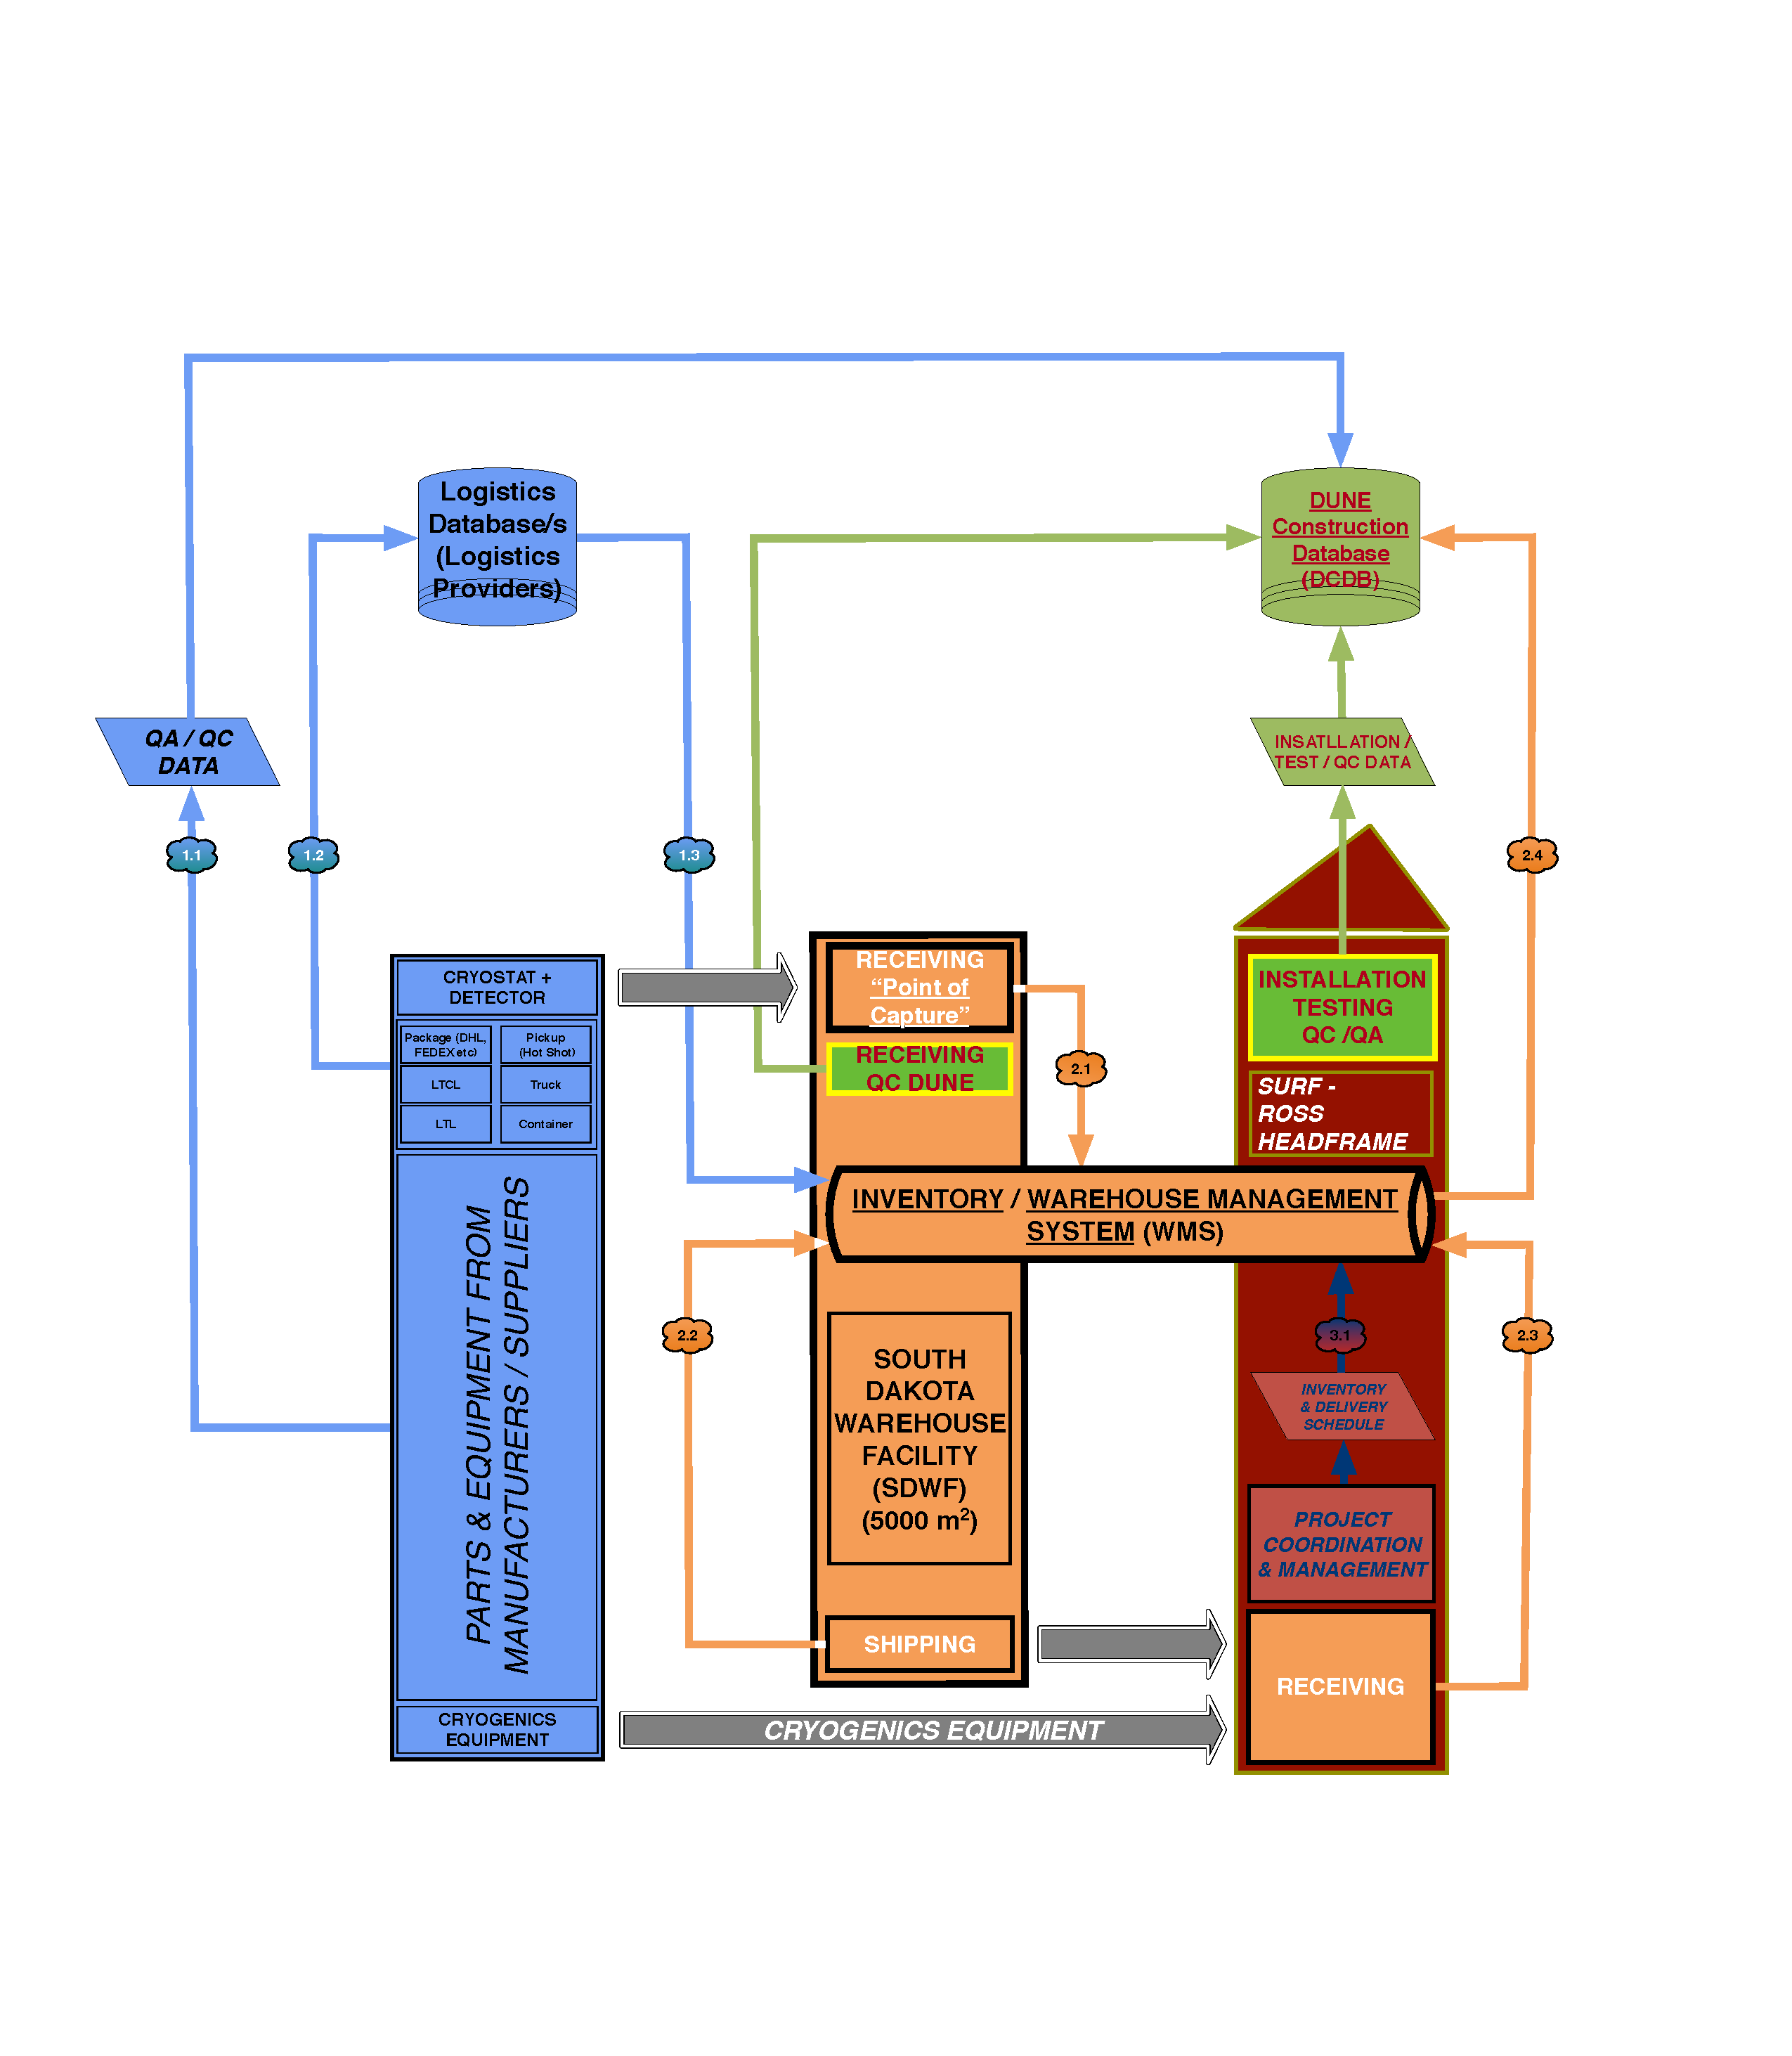
\includegraphics[width=\textwidth]{logistics-data-and-mat-flow}
\end{dunefigure}

 
The \dword{jpo} installation management team will provide a shipping (supply) report to the \dword{sdsd} logistics organization and \dword{sdwf} for scheduling delivery of parts and equipment two weeks in advance of the required delivery date. 
All deliveries will be inventoried upon receipt at the Ross Headframe in the \dword{wms}. 




%%%%%%%%%%%%%%%%%%%%%%%%%%%%
\subsection{Logistics Safety}
\label{sec:fdsp-tc-log-safety}


The \dword{sdwf} will be managed and operated by an independent contractor under the supervision of the logistics manager. 

The facility will be operated under the contractor's \dword{esh} program that has to conform to federal regulations and will be reviewed by \dword{fnal}'s \dword{esh} management prior to entering a contractual relationship.